\section{Objectifs pour la deuxième soutenance}
\noindent Voici la répartition prévue des tâches entre les étudiants du groupe gameHUB pour la deuxième soutenance.

\subsection{Sauvegardes}
\setlength{\parindent}{5ex}
Concernant les sauvegardes, nous avons décidé de placer des bornes de sauvegarde, représentées par une ancienne radio, qui serons placé à des endroit stratégique du jeu. Cette mécanique permet de simplifier le système de sauvegarde car ne demande pas de connaître l’emplacement du joueur et rendra le jeu plus stressant, car empêche le joueur de sauvegarder sa progression à tout instant.
\begin{figure}[H]
\centering
\begin{minipage}{.5\textwidth}
  \centering
  \centerline{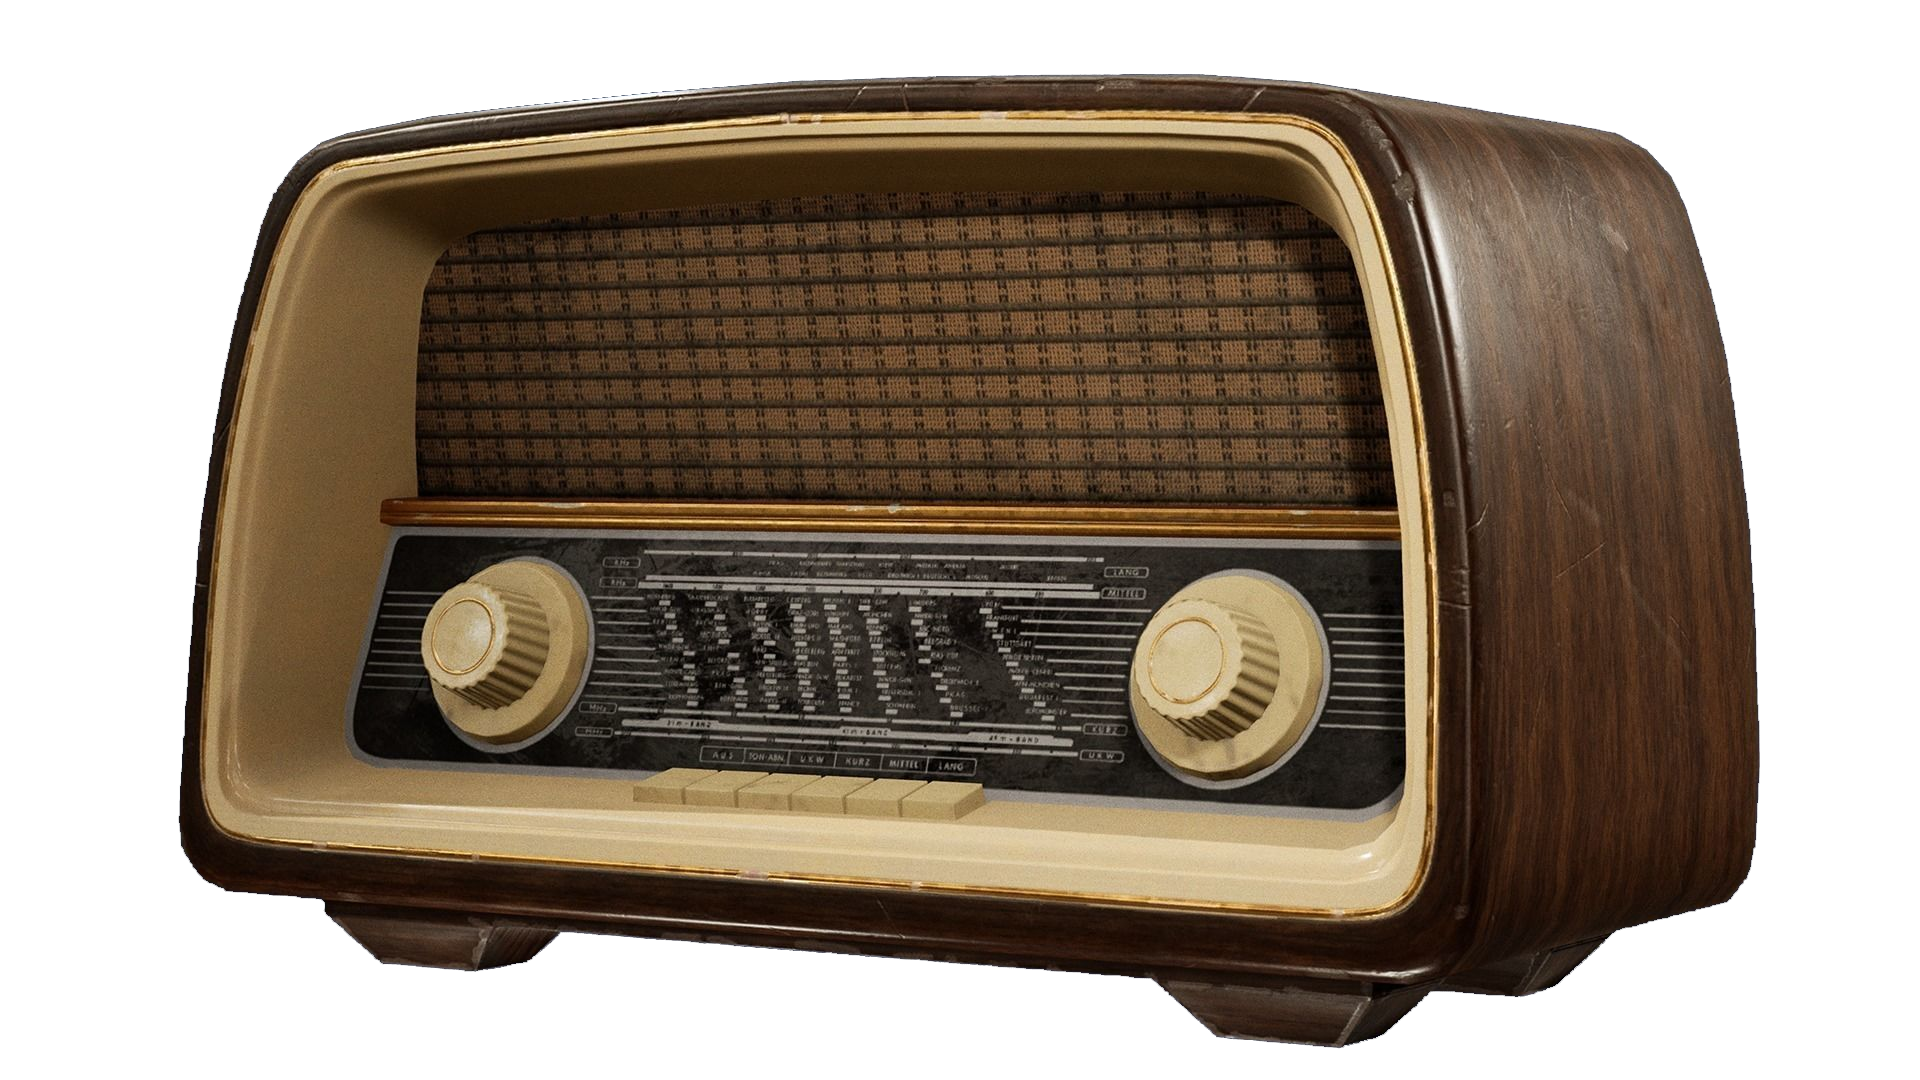
\includegraphics[width=1.5\linewidth]{img/assets/save.png}}
  \captionof{figure}{\emph{Borne de sauvegarde}}
  \label{fig:save}
\end{minipage}%
\end{figure}
\newline

Concernant les contrôles enjeu, nous devrons aussi implémenter une touche d’action pour interagir avec les objets du jeu, tel que des portes, des bornes de sauvegarde ou des objets en notre possessions nécessaire à l’avancé du jeu. Ceci nous demandera aussi de définir la portée d’action du personnage.
L'ajout de l'apparition du menu lors de l'appui sur la touche ``escape'' doit aussi être implémenté.
\newline

\vfill
\noindent\makebox[\linewidth]{\rule{.8\paperwidth}{.6pt}}\\[0.2cm]
EPITA Toulouse - Projet S2 - 2022 \hfill Nyctalopia - gameHUB
\noindent\makebox[\linewidth]{\rule{.8\paperwidth}{.6pt}}

\newpage

Le script, servant à redéfinir les touches de contrôles, n’est pas encore terminé, certains cas ne sont pas pris en compte, notamment le fait de d’empêcher le joueur d’assigner la même touche à plusieurs actions. Nous allons aussi devoir, par la suite, adapter ce script pour l’ajouter au menu en jeu. Le script peut déjà être adapté pour la touche « utiliser », qui seras implémentée plus tard.
Une sauvegarde des touches redéfinies doit aussi être implémentée.

\subsection{Gameplay}

Concernant le gameplay, nous avons déjà commencé à réfléchir à certaines énigmes telle que la récupération de fusibles pour ouvrir des portes débloquant ainsi la suite de l’histoire.
\newline

\begin{figure}[H]
\centering
\begin{minipage}{.5\textwidth}
  \centering
  \centerline{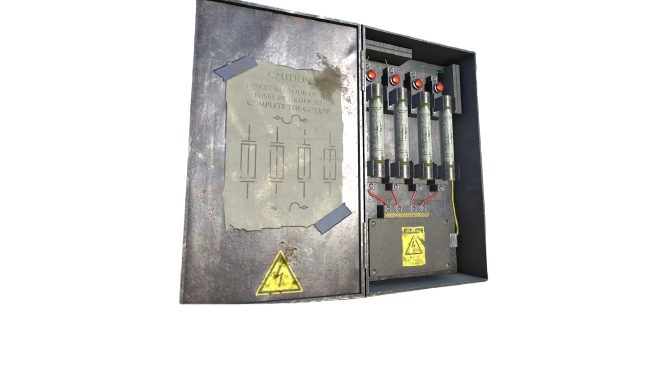
\includegraphics[width=1.5\linewidth]{img/assets/fusibles.png}}
  \captionof{figure}{\emph{Boîte à fusibles}}
  \label{fig:fusebox}
\end{minipage}%
\end{figure}

\subsection{Map}

Nous envisageons aussi l'introduction d'une nouvelle zone de jeu: les égouts. Cette zone sera réalisée à l'aide de bibliothèques 3D dédiées à la conception de chambres et couloirs modulaires.

\vfill
\noindent\makebox[\linewidth]{\rule{.8\paperwidth}{.6pt}}\\[0.2cm]
EPITA Toulouse - Projet S2 - 2022 \hfill Nyctalopia - gameHUB
\noindent\makebox[\linewidth]{\rule{.8\paperwidth}{.6pt}}

\newpage

\begin{figure}[H]
\centering
\begin{minipage}{.5\textwidth}
  \centering
  \centerline{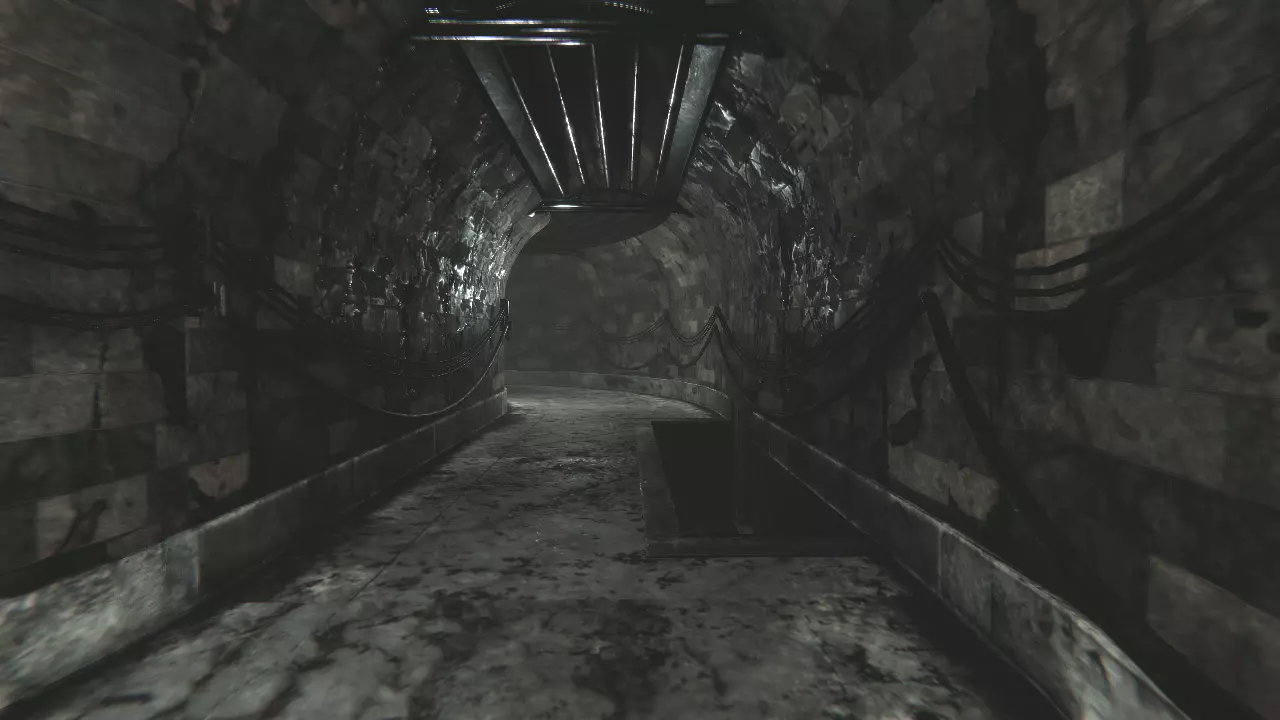
\includegraphics[width=1\linewidth]{img/assets/egouts1.png}}
  \captionof{figure}{\emph{Aperçu des égouts}}
  \label{fig:fusebox}
\end{minipage}%
\end{figure}

\subsection{Communication}

Nous avons prévu de changer la police d'écriture temporaire du logo du jeu Nyctalopia (actuellement : ``\emph{Venom}'') vers la police ``\emph{October} Crow''.

\begin{figure}[H]
\centering
\begin{minipage}{.5\textwidth}
  \centering
  \centerline{
\includegraphics[width=1.5\linewidth]{img/font.png}}
  \captionof{figure}{\emph{Police d'écriture choisie pour Nyctalopia}}
  \label{fig:octobercrowfont}
\end{minipage}%
\end{figure}

\vfill
\noindent\makebox[\linewidth]{\rule{.8\paperwidth}{.6pt}}\\[0.2cm]
EPITA Toulouse - Projet S2 - 2022 \hfill Nyctalopia - gameHUB
\noindent\makebox[\linewidth]{\rule{.8\paperwidth}{.6pt}}

\newpage